\documentclass[a4paper,11pt]{article}
\usepackage[a4paper,left=0.99in, right=0.99in,top=1.2in, bottom=1.2in]{geometry}

\usepackage{hyperref}
\usepackage{listings}
\usepackage{courier}
\usepackage{caption}
\usepackage[dvips]{graphicx} % has to be before color and xcolor packages
\usepackage{color}
\usepackage{xcolor}
\DeclareCaptionFont{white}{\color{white}}
\DeclareCaptionFont{black}{\color{black}}
\DeclareCaptionFormat{listing}{\colorbox{lightgray}{\parbox{\textwidth}{#1#2#3}}}
\captionsetup[lstlisting]{format=listing,labelfont=black,textfont=black}
%\numberwithin{equation}{section}


\lstset{
         basicstyle=\small \ttfamily, % Standardschrift
         %numbers=left,               % Ort der Zeilennummern
         numberstyle=\tiny,          % Stil der Zeilennummern
         %stepnumber=2,               % Abstand zwischen den Zeilennummern
         numbersep=5pt,              % Abstand der Nummern zum Text
         tabsize=2,                  % Groesse von Tabs
         extendedchars=true,         %
         breaklines=true,            % Zeilen werden Umgebrochen
         keywordstyle=\color{red},
            frame=b,         
 %        keywordstyle=[1]\textbf,    % Stil der Keywords
 %        keywordstyle=[2]\textbf,    %
 %        keywordstyle=[3]\textbf,    %
 %        keywordstyle=[4]\textbf,   \sqrt{\sqrt{}} %
         stringstyle=\color{white}\ttfamily, % Farbe der String
         showspaces=false,           % Leerzeichen anzeigen ?
         showtabs=false,             % Tabs anzeigen ?
         xleftmargin=17pt,
         framexleftmargin=17pt,
         framexrightmargin=5pt,
         framexbottommargin=4pt,
         %backgroundcolor=\color{lightgray},
         showstringspaces=false      % Leerzeichen in Strings anzeigen ?        
}


\title{IdSolver notes}
%\author{Sebastian Sapeta}
%-----------------------------------------------------------------------------
\begin{document}
\maketitle

\noindent \rule{\textwidth}{1pt}
\tableofcontents
\noindent \rule{\textwidth}{1pt}

\newpage

%-----------------------------------------------------------------------------
\section{General guidelines}


\begin{itemize}
  \item
  \verb+lorentz3p.prc+ is needed for 3-point functions\\
  \verb+lorentz4p.prc+ is needed for 4-point functions
  \item
  Edges in prototype file must be declared following some convention.
  \item
  Temporary \verb+form+ files are stored as \verb+.number.id.frm+. The
  corresponding \verb+form+ log file in \verb+.number.id.log+.
\end{itemize}

%-----------------------------------------------------------------------------
\section{Tools directory}

%-----------------------------------------------------------------------------
\subsection{generate\_identities}

\begin{verbatim}
  ./generate_identities prototype nscalars ndeno d n symbols
\end{verbatim}

\begin{itemize}
  \item
  \verb+prototype+: name of the prototype
  \item
  \verb+nscalars+: number of indices \verb+n1, n2,...nscalars+
  \item
  \verb+ndeno+: number of denominators; notice that \verb+nscalars >= ndeno+
\end{itemize}

Contrary to its name, this program requires the full set of administrative files
(symmetries, matchings, identities, integrals, kinematics, etc.). What it does
is the following It applies IBPs, which are stated in general in those files, in
particular in \verb+PR?identities.prc+, to a concrete set of integrals specified
by the command line arguments, {\it i.e.} integrals with specific indices.
%
The result ends up in \verb+idprototype.dat+ and \verb+PR?inc.dat+ files are
created as well. All these are binary database files that contain IBPs, LIs
etc. in the FORM format, which look like this

\begin{verbatim}
  id4 = 
      + PR0(1,2,1) * ( - 1/2 )
      + PR0(1,2,2) * ( 1/2 )
      + PR0(2,1,1) * ( 1/2 )
      + PR0(2,1,2) * ( - 1/2 );
\end{verbatim}


%-----------------------------------------------------------------------------
\subsection{solve\_integrals}

\begin{verbatim}
  ./solve_integrals integrals output symbols
\end{verbatim}


\begin{itemize}
  \item
   \verb+integrals+: file with list of integrals in the format like
   \verb+PR1(3,0,0)+
  \item
   \verb+output+
  \item
   \verb+symbols+: usual \verb+ep+
\end{itemize}

This program will use databases created by \verb+generate_identities+ and
will generate \verb+fill+ statements (like Substitutions file from the
\verb+solve_prototypes+). Depending on what is found the input databases, the
output will be more or less simplified.


%-----------------------------------------------------------------------------
\subsection{read\_identities}

\begin{verbatim}
  ./read_identities prototype begin end firstid symbols
\end{verbatim}

Read identities stored in FORM log files. The files need to be called as:
\verb+0.log+, \verb+1.log+... \verb+n.log+. Then, \verb+begin+ and \verb+end+
are the starting and ending numbers of the set of files that should be read.
\verb+firstid+ is the number of the identity we want to start from.

%-----------------------------------------------------------------------------
\subsection{print\_identities}


\begin{verbatim}
  ./print_identities prototype output
\end{verbatim}

Print identities stored in \verb+idprototype.dat+ database and print them in the
text formatn into the  \verb+output+ file.

%-----------------------------------------------------------------------------
\section{test directory}

This directory contains an example, which can be run as
%
\begin{verbatim}
  $./solve_prototypes proto 1 1 ep
\end{verbatim}
%
\verb+ep+ above means $\epsilon$. The two numbers mean the sum of denominator
and numerator powers.

Options:  

\begin{tabular}{ll}
  \verb+-p+ & prints postscript pictures for all the prototypes \\
  \verb+-v+ & verbose
\end{tabular}

This will produce the file \verb+Substitutions+ that contains all the simplified
\verb+fill+ statements and the file \verb+Masters+ with all the masters.

Exactly the same effect can be achieved by the following sequence

\begin{verbatim}
    $ ./generate_identities PR0 3 3 1 1 ep
    $ ./generate_identities PR1 3 1 1 1 ep
    $ ./generate_identities PR2 3 2 1 1 ep
    $ ./generate_identities PR3 3 2 1 1 ep

    $ ./solve_integrals  inputint out ep

    $ ./determine_masters PR0 3 3 1 1 1 1 ep
    $ ./determine_masters PR1 3 1 1 1 1 1 ep
    $ ./determine_masters PR2 3 2 1 1 1 1 ep
\end{verbatim}
%
The masters that come out in stdout will be exactly those from \verb+Masters+
and the file \verb+out+ will be identical with \verb+Substitutions+.


%-----------------------------------------------------------------------------
\subsection{determine\_masters}

\begin{verbatim}
usage: ./determine_masters [-n] [-f prototypes | prototype nscalars 
        ndeno d n] dm nm symbols
\end{verbatim}


This program does not need databases of integrals. It only needs FORM procedures
like 
\verb+PR0identities.prc+, \verb+PR0symmetries.prc+ and corresponding include
files. Witn \verb+nscalars+ = \verb+ndeno+ the value of \verb+n+, the maximal sum of
numerators is irrelevant.



%-----------------------------------------------------------------------------
\subsection{Input files}

%------------------------------------
\subsubsection*{proto}

\begin{figure}[t]
  \begin{center}
    \begin{minipage}[h]{0.25\textwidth}
    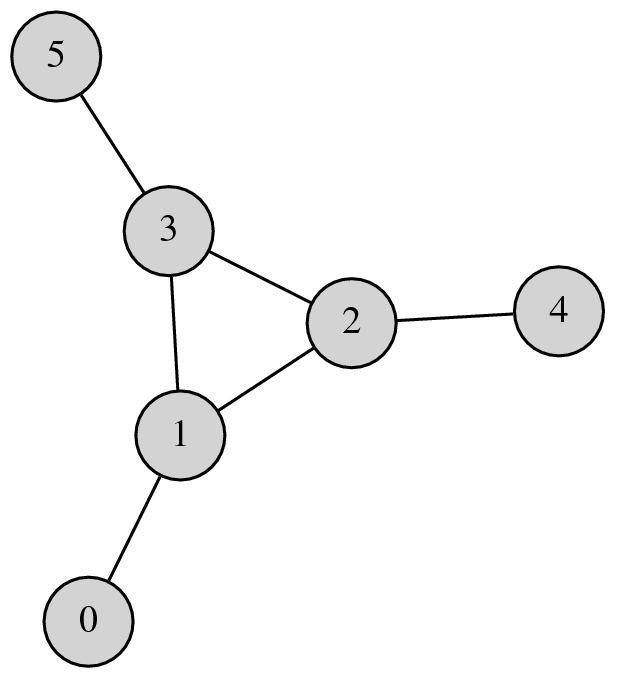
\includegraphics[width=\textwidth]{plots/PR0.png}
    \end{minipage}
    \hspace{100pt}
    \begin{minipage}[h]{0.25\textwidth}
    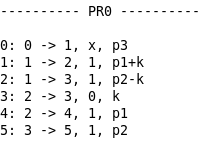
\includegraphics[width=\textwidth]{plots/PR0print.png}
    \end{minipage}
  \end{center}
  \caption{
  {\it Left:} Graphical representation of the prototype {\tt PR0}.
  %
  {\it Right:} The actual content of {\tt PR0} obtained by printing the
  {\tt PrototypeMap} object. The left column is the node name, then the edges
  connecting the nodes, then the masses of the lines and then the 4-momenta of
  the lines.
  %
  Printout on the r.h.s. comes from temporary {\tt form} files created and used
  by {\tt IdSolver}.
  }
  \label{fig:PR0}
\end{figure}

As shown in the example below, diagrams are specified by setting the number of
nodes \verb+n+, then \verb+e+ $ni\ nj$ describes the edges between nodes $ni$
and $nj$.
%
The lines \verb+m -p1 4+  specifies the momentum $p1$ on edge 4 and outgoing.


\begin{lstlisting}[label=test-proto, caption=proto]
n 6     # number of nodes
e 0 1 x # edge from node 0 to node 1 with mass x
e 1 2 1
e 1 3 1
e 2 3 0
e 2 4 1
e 3 5 1
m +p3 0 # ingoing external momentum p3 on edge 0
m -p1 4 # outgoing external momentum p1 on edge 4
m -p2 5
\end{lstlisting}

The above listing corresponds to the configuration shown in Fig.~\ref{fig:PR0}.
The nodes are marked with circles and the edges correspond to lines connecting
the circles. The incoming/outgoing momenta are themselves the edges. The RHS of 
Fig.~\ref{fig:PR0} is what is in the actual \verb+Prototype+ object graphically
represented on the LHS.

The diagram from Fig.~\ref{fig:PR0} is a triangle. Three of the edges
correspond to propagators and three other to the external particles.

%------------------------------------
\subsubsection*{userkinematics}

That file contains kinematic identities. Comments with \# are not recognized.

\begin{lstlisting}[label=test-userkinematics, caption=userkinematics]
id p1.p1 = 0;
id p2.p2 = 0;
id p1.p2 = 1/2;
\end{lstlisting}

%------------------------------------
\subsubsection*{ibp.prc}

\begin{itemize}
  \item
  \verb+SS+ functions are the scalar products.
\end{itemize}

%-----------------------------------------------------------------------------
\subsection{Output files}

%------------------------------------
\subsubsection*{Masters}

Here is where the set of master integrals ends up. The prototypes are called
with the names going like \verb+PR?+.

\begin{lstlisting}[label=test-Masters, caption=Masters]
PR1(1,0,0)
PR2(1,1,0)
PR0(1,1,1)

3 master integral(s) identified
\end{lstlisting}

\subsubsection*{Substitutions}

Integrals expressed in terms of masters like for example
%
\begin{lstlisting}[label=test-Substitutions, caption=Substitutions]
fill PR0(1,1,2) =

 + PR0(1,1,1) * (ep)

 + PR1(1,0,0) * (2*ep-2)

 + PR2(1,1,0) * (-2*ep+1)
;

\end{lstlisting}

%-----------------------------------------------------------------------------
\section{The code}

\subsubsection*{PrototypeMap.cpp: PrototypeMap::insert(NamedPrototype* p)}

This is one of the main functions, where a lot is being done. In particular, all
the prototypes are derived here.

\subsubsection*{DiaGen/Prototype.cpp}

The original \verb+Prototype+ class is defined in \verb+DiaGen+.

\subsubsection*{IdentityGenerator::StoreIdentities}

If this option is set identities are saved in databases. This option is enabled
by (hard coded) in \verb+generate_identities+ and can be chosen at run time in 
\verb+solve_prototypes+ with the command line argument \verb+-c+.

\subsubsection*{decls}

Prototypes like \verb+PR0(n1,n2,n3)+ are effectively sparse tables where the
table indices run over indices of the topology.

\subsubsection*{SolveNumerators}

It is a switch in \verb+IdSolver.hpp+. When set to 0, results will contain
irretudible numerators, when set to 1, those numerators are solved into masters
with dots (double denominators).

%-----------------------------------------------------------------------------
\subsection*{Errors}

\begin{itemize}
  \item
  When the program gets stuck at
  \verb+Creating administrative and identity files...+
  most probably, the path to \verb+fermat+ is not correct
  \item
  Some errors end up in the files \verb+PR?identities.prc+ and in the variable
  \verb+current_identity+ of \verb+IdentityGenerator.cpp+.

\end{itemize}


%-----------------------------------------------------------------------------
\bibliographystyle{unsrt} % sorts in the order of apperance
\bibliography{}

\end{document}
